\chapter{Designing the methods and UX/UI research}\label{ch:A}
\section{General description}
\par
Actually, UX design sphere consists of some constituent elements like design usability, accessibility, comfortability, design system performance and testing. In this thesis I would talk about some of them like visual concepts, usability and in common design. Exactly, such thoughts about behavior and understanding of the user on web pages should be noted, which is very important in comfort for people. The process on the part of the user is very important here, since the project is intended for people of all ages and the research will help in the further implementation of the project. 
\par
For a good design to make a product befit, designers learn from their users how to do it using a variety of techniques and techniques in the UX industry. It is unique for each project.
\par
The project was not easy, the task was to create a website that will serve as an entrance to the world of donation, which includes completely different content that distinguishes it from all others, the one and only. My task was to implement a new design for desktop and mobile versions of the website to make it adaptive.
\par
A design system was used to superimpose interactions within the project, reference point and structure. Naturally, the project is clean from scratch, so the best solution was to make a list of all the different templates, colors, text styles and patterns that we use in our design \cite{eyal}. We started experimenting with some visual patterns like initial UI elements, layouts. The creation of various concepts and chose the most promising ones. 
\par
The usage of the principles of atomic design allowed to develop not only attracting interface, but also a system that is logically structured. As mentioned earlier, we started with some particles like colors, fonts, shapes. Moving on to atoms, buttons, inputs, containers and pagination from scratch of the construction is a method of designing a good usable interface. Finally, we made up the molecules - the search field, date-address pickers, navigation bars, side menus and organisms - lists, registration containers. Due to this, we were able to prepare templates for element pages -  our own UI kit system which has unique style and independent logic. 


\section{Design development and processing}
\par
When creating a project from scratch, the first idea and the process itself started from the main step - thinking \cite{eyal}. Thinking about the design began with drawing on a piece of paper. We had a few thoughts on how to implement the 'Donor project' design. The most important thing at that moment was to write down all the thoughts, even if they were good or bad. The general ideas were already established when we were stating the problems of current donation process and having collected it all into one we could begin working on further development of the idea, depending on our main aims and goals, such as simple interface but good logical construction. (see Figure \ref{fig:main})
\begin{figure}[h]
    \centering
    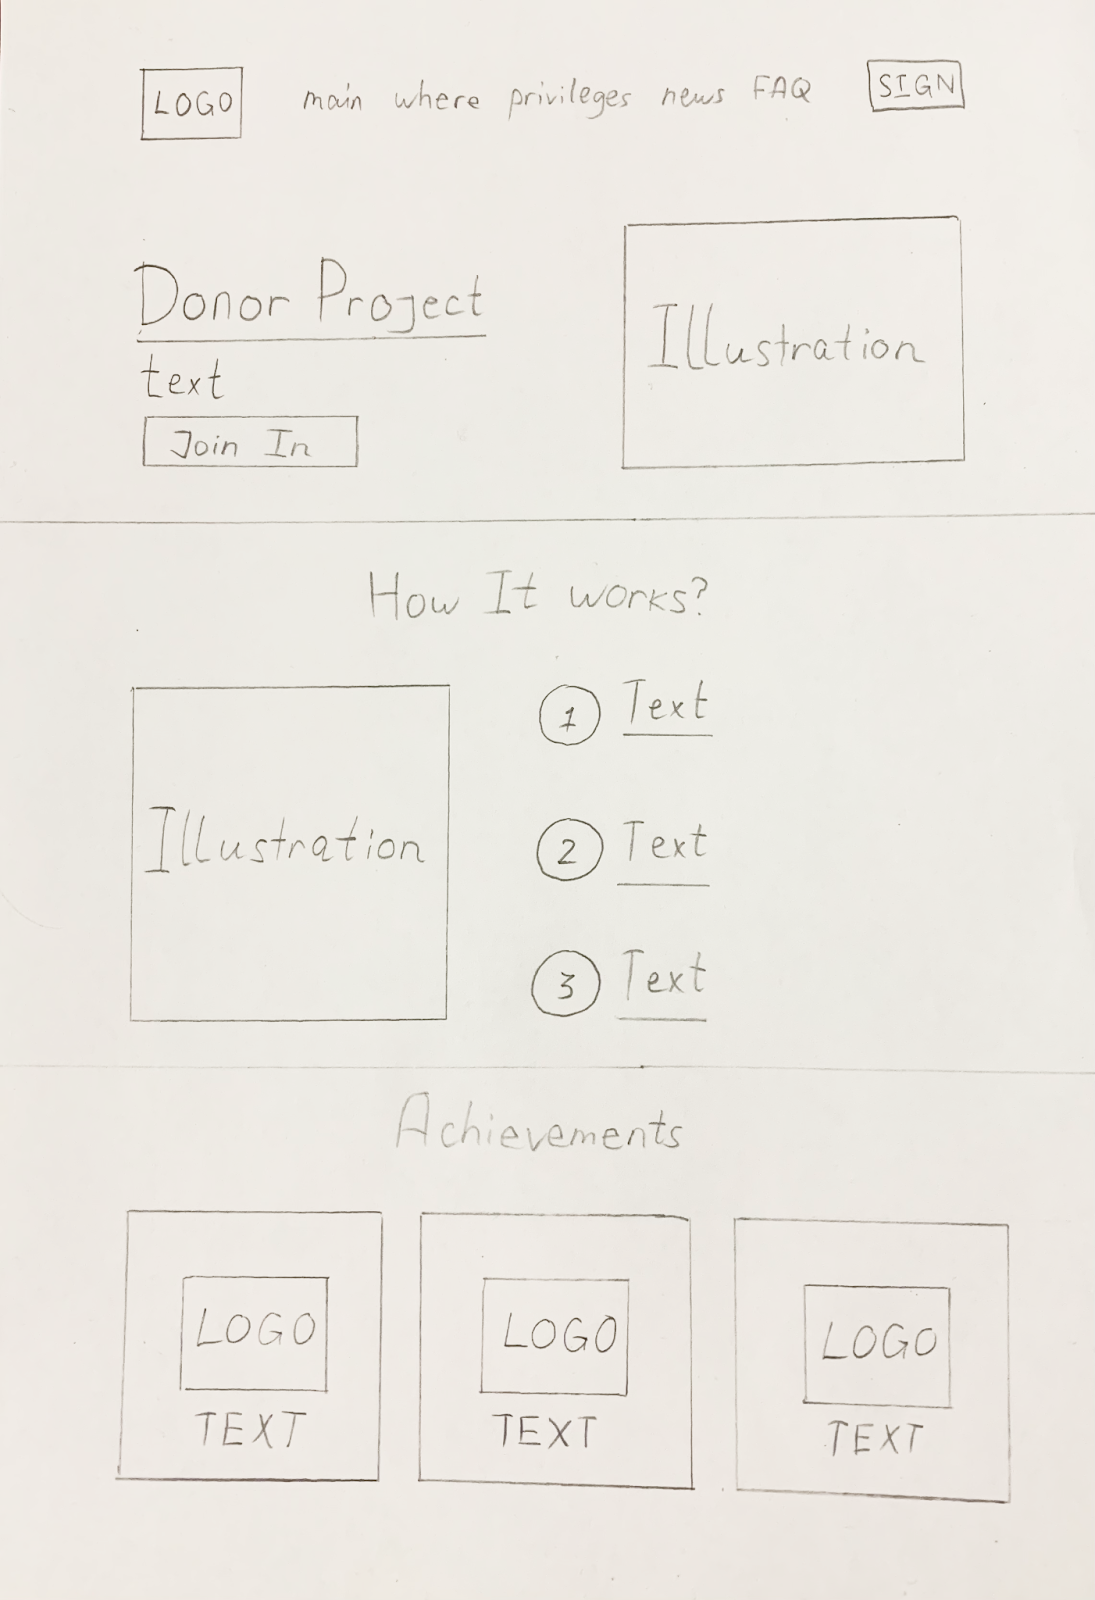
\includegraphics[scale=0.18]{figures/1.png}
    \caption{Sketch of the Main Page}
    \label{fig:main}
\end{figure}
To integrate, firstly researches were made on websites for competitive-promoting companies that are related to our market, looking at their designing and analyzing the idea behind it we got  more familiar with the donation industry. This gave a better understanding of how the pages on the donation site should look like. Writing down and memorizing best and bad practice became handy in the further design of the project and using other people's experience helped to develop better system \cite{martinez}. 
\par
Almost all sites that were used for research had main pages such as: a profile page, a question and answer page, a contact page.
After long deliberation over the pages that the 'Donor project' will have, the decision came to the general idea: Home, Where to donate blood, privileges, and FAQ. They served as the main pages in our header which conduct as a map of the website that will be developed.
\par
The name of the project and its description are in the first place. This is used on almost every site to show the user what the company is.
After the name of the company, the decision to present the company in the section how it works and the section footer.
Potential clients usually want to see the result of the company's work and what they are capable of \cite{martinez}. In this case, clients are potential donors of different ages. Therefore, the best solution is to provide the client with all the information about the project and what it represents. (see Figure \ref{fig:profilesketch})
\begin{figure}[h]
    \centering
    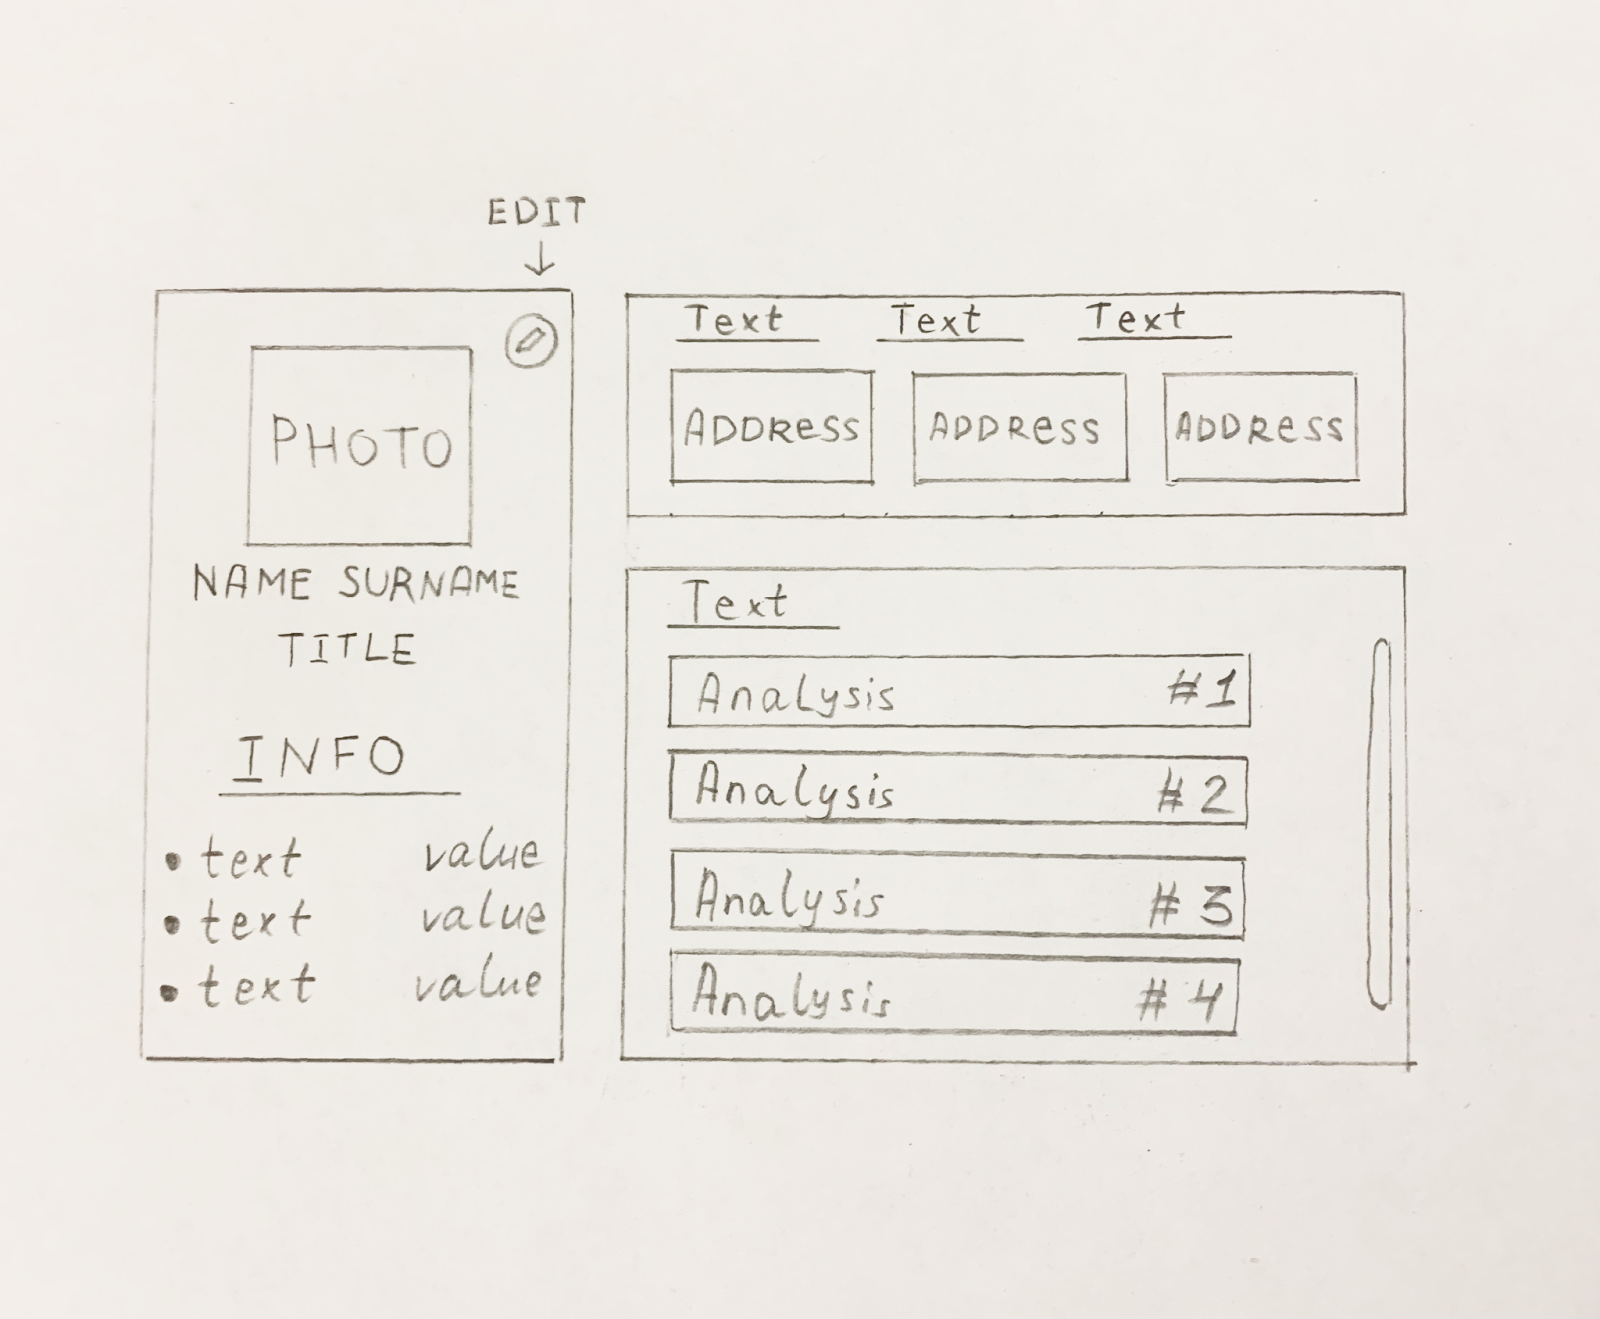
\includegraphics[scale=0.2]{figures/2.png}
    \caption{Sketch of the User profile}
    \label{fig:profilesketch}
\end{figure}
\par
The idea behind this profile page is to provide the user with unique information about them in one place. This page has several navigation that is different from the information that a regular unauthorized client owns. The sketch shows the initial ideas such as profile information on the side and information containers. The latest update will include tests and blood donation records. The purpose of a location with information about the profile is explained by the fact that it was necessary to make it larger for good visibility and on the left, since the user entering the page sees the elements on the left at the beginning. The information can change depending on the user. If you wish, you can change information about yourself by clicking on the edit button.

\section{Implementation of visual design and usability}
Usability testing made it possible to obtain information about how the user interacts with the site and, in general, to find out behavior. It took a long time to analyze user flows and  understand the importance of a completely new project design which doesn't have analogues. 
\par
After creating sketches and wireframes,it was necessary to start design scratches in order to implement the next part of the project, which is the design itself and its visualization. The value of visualization reveals the identity of the brand. For this, there were used the concepts and sketches prepared earlier. The visual implementation was changing several times so that the best practice for our product could be achieved. In Figma prototypes of the project is shown the process of the implementation, which demonstrates step by step changes depending on the user needs which were gathered throughout the project development.
\par
In general, the main goal is to create an interactive and user-friendly design with its own note of uniqueness for the donor project. The main tools of the designer helped in uniqueness. Coloristics, typography and fonts and interaction details were the most important aspects for us during the process of designing the website.

\section{Illustrations}
All illustrations that are on the pages are drawn by hand and they are also associated with blood. It was important not only to include unique content but to make it meaningful and eye-catching for the user, so that in future if some of our picture may be seen they will be immediately associated with the brand of 'Donor project'.
\par
An example of illustration shows test tubes with blood and a person sitting on the phone, showing us the mobility of the project and the interaction of medicine with technology. (see Figure \ref{fig:mainillustration})
\begin{figure}[h]
    \centering
    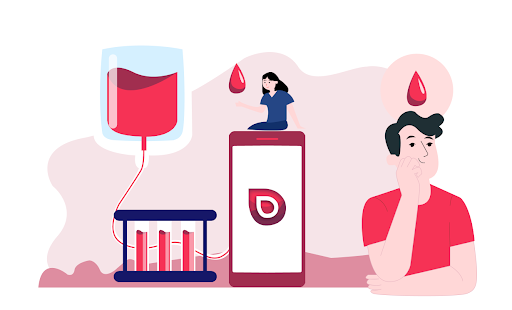
\includegraphics[scale=0.7]{figures/3.png}
    \caption{Illustration on the Main page}
    \label{fig:mainillustration}
\end{figure}

\section{Color scheme}
The goal is to create a simple, but at the same time to show in the design colorfulness and professionalism, expressed by confidence, emotions and even aroused desire among potential customers and users. 
\par
As we know, the donor project has a theme of medicine and blood, therefore, as studies of similar institutions and projects have shown, it is worth choosing colors associated with this area. Undoubtedly, the primary color was chosen for the page design is red. For a change, having played with the palette, we brought out several auxiliary colors. 
\par
The background itself is white for neutrality and visibility of key visual elements. The text received several shades: black, gray and shades of red. Black, white and gray are neutral colors. Neutral colors usually create a backdrop in design. They can be used on their own, or combined with another color accent. Black color was used for typography and other functional elements because of its neutrality. (see Figure \ref{fig:colorscheme})
\begin{figure}[h]
    \centering
    
\includegraphics[scale=0.5]{figures/4.png}
    \caption{Color Scheme}
    \label{fig:colorscheme}
\end{figure}
\par
White stands for purity and kindness. And the use of red is generally an art, since it is different and popping. It is the color of strength, so it can show irritability, anxiety, and even anger. But with the correct mixing of shades, in our case, frankness, love and confidence are shown.
The usage of white for the background and black for the text is a common technique that creates contrast between text and background and highlights other shades of elements on the site.

\section{Typography and fonts}
For the design there were used the fonts with good readability. The fonts do not contain additional elements, which can cause difficulties in recognizing the letters and slow down the speed of reading the text. Size of the font is big enough for comfortable reading. The font has no extra characters or serifs. Gilroy was chosen for the font. This font has twenty styles but its structure is very simple, therefore it is trendy today and fits well with design idea. (see Figure \ref{fig:font})
\par
As mentioned before in section of color significance, the text colors were based on black and shades of red. White and gray are used in dark places, there is no unreadable text in any place of the site, everywhere its own harmony. But black was replaced by dark red according to design measures. All this for easy reading and quick perception of the text. 
\par
\begin{figure}[h]
    \centering
    
\includegraphics[scale=0.5]{figures/5.png}
    \caption{Text-font example}
    \label{fig:font}
\end{figure}

\section{Interactive elements}
For the website version, we decided to add more motion and animations to attract the user. When swiping over the elements of the page, the user can see that most of the elements interact well with the user. Added animations, hovers on buttons, that is, they become moving and highlighted. On the main page, site visitors can see a slider with achievements that are also made by hand.
\begin{figure}[h]
    \centering
    
\includegraphics[scale=0.5]{figures/10.png}
    \caption{Buttons hover}
    \label{fig:buttons}
\end{figure}
\par
After logging in and viewing the achievements, illustrations were made with different logos of a certain achievement. Made in two styles to distinguish which achievements have been achieved and which have not yet been achieved. If there is a certain achievement, it will be filled and colored in red shades. 
\par
The uniqueness of the illustration also develop a habit of engagement in people's minds so that everything that is developed will be memorized by users. Aim was to be memorized, this will create strong association with the 'Donor project' and in future it will be much more easier to advertise the product.
\begin{figure}[h]
    \centering
    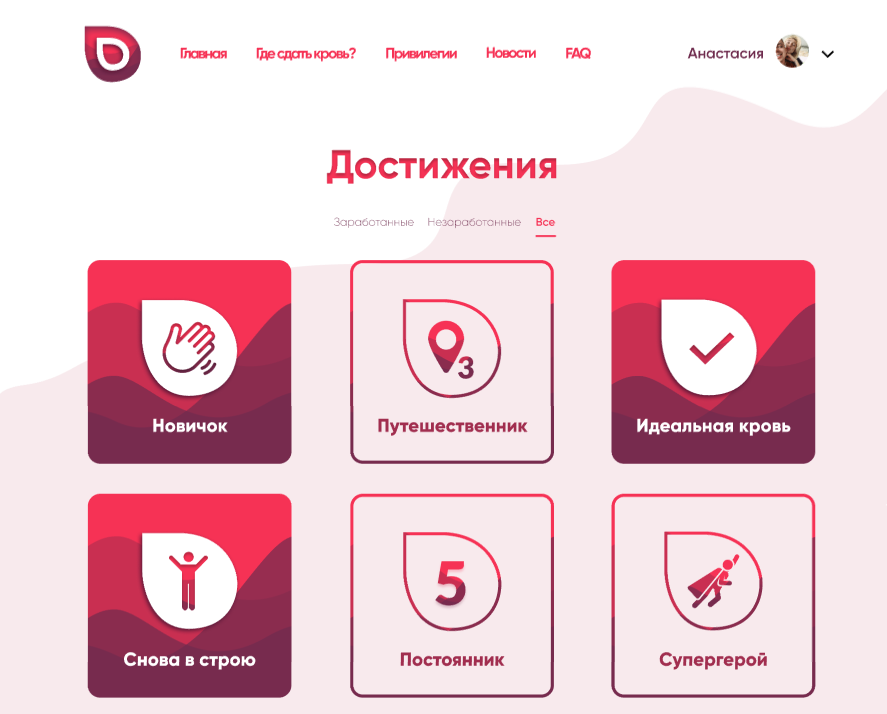
\includegraphics[scale=0.45]{figures/11.png}
    \caption{Text-font example}
    \label{fig:interactive}
\end{figure}




